% elementos pós-textuais 
%\postextual

% apêndice 
\begin{apendicesenv}
\partapendices

% Apêndice A
\chapter{DERIVAÇÃO DOS ESTIMADORES DE MQO} \label{apendice_mqo}

Partindo de um modelo de regressão linear simples, $Y_i = \beta_0 + \beta_1X_i + e_i$, em que $e_i$ é o termo de erro estocástico, em uma amostra, a relação $Y$ e $X$ é dada por:

1. Função de regressão amostral
\begin{equation}
Y_i = \hat{\beta}_0 + \hat{\beta}_iX_i + \hat{e}_i
\end{equation}

2. O valor $Y_i$ previsto pelo ajuste
\begin{equation}
\hat{Y}_i = \hat{\beta}_0 + \hat{\beta}_iX_i
\end{equation}

3. O resíduo $\hat{e}_i$ não previsto pelo ajuste
\begin{equation}
\hat{e}_i = Y_i - \hat{Y}_i
\end{equation}

% incluir figura
\begin{figure}[H]
\centering
\caption{Resíduos da regressão linear}
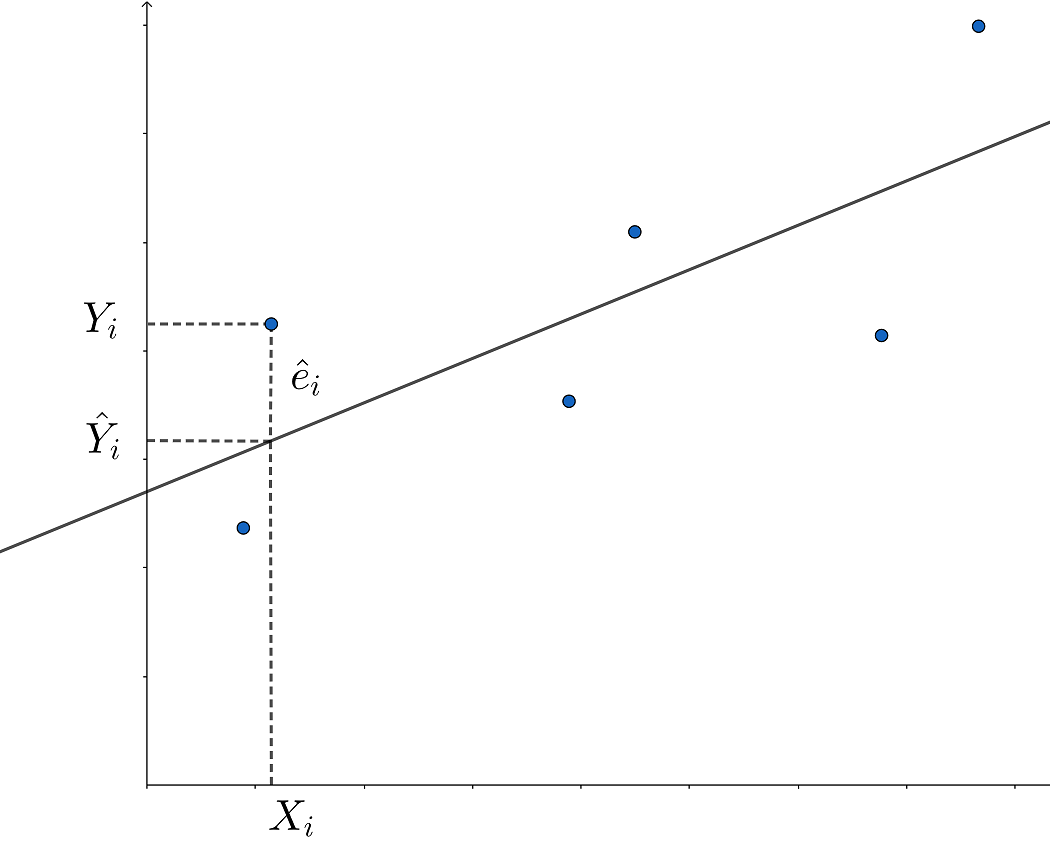
\includegraphics[width=0.7\textwidth]{img/appendix_b_1.png}
\caption*{Fonte: Elaboração própria}
\end{figure}

O objetivo é, portanto, estimar os coeficientes linear e angular que representam a reta que minimiza os resíduos. Para essa função a ser minimizada, posso utilizar tanto o erro absoluto $\mid \hat{e}_i \mid$ quanto o erro quadrático $\hat{e}_i^2$. Por simplicidade, opto pelo erro quadrático total.

\begin{equation}
\begin{aligned}
\text{EQT} & = \hat{e}^2_1 + \hat{e}^2_2 + ... + \hat{e}^2_n \\
& = (Y_1 - \hat{Y}_1)^2 + (Y_2 - \hat{Y}_2)^2 + ... + (Y_n - \hat{Y}_1)^2 \\
& = \sum_{i=1}^{n}(Y_i - \hat{Y}_i)^2 \\
& = \sum_{i=1}^{n}[Y_i - (\hat{\beta}_0 + \hat{\beta}_iX_i)]^2
\end{aligned}
\end{equation}

De posse da função, posso minimizar os coeficientes $\beta_i$. Considerando um modelo de regressão simples, posso estimar $\beta_0$ e $\beta_1$ igualando as derivadas parciais à zero.

\begin{equation}
\begin{aligned}
\frac{\partial \text{EQT}}{\partial \beta_0} & = 2\sum_{i=1}^{n}[Y_i - (\hat{\beta}_0 + \hat{\beta}_1X_i)] (-1) & = 0 \\
& = -2 (\sum_{i=1}^{n} Y_i - \sum_{i=1}^{n} \hat{\beta}_0 - \sum_{i=1}^{n} \hat{\beta}_1X_i) & = 0 \\
& = \sum_{i=1}^{n} Y_i - n\hat{\beta}_0 - \hat{\beta}_1 \sum_{i=1}^{n} X_i & = 0 \\
& n\hat{\beta}_0 = \sum_{i=1}^{n} Y_i - \hat{\beta}_1 \sum_{i=1}^{n} X_i \\
& \hat{\beta}_0 = \frac{\sum_{i=1}^{n} Y_i - \hat{\beta}_1 \sum_{i=1}^{n} X_i}{n}
\end{aligned}
\end{equation}

\begin{equation}
\begin{aligned}
\frac{\partial \text{EQT}}{\partial \beta_1} & = 2\sum_{i=1}^{n}[Y_i - (\hat{\beta}_0 + \hat{\beta}_1X_i)] (-X_i) & = 0 \\
& = -2X_i (\sum_{i=1}^{n} Y_i - \hat{\beta}_0\sum_{i=1}^{n} - \hat{\beta}_1\sum_{i=1}^{n} X_i^2) & = 0 \\
\end{aligned}
\end{equation}


\end{apendicesenv}

% anexos 
%\begin{anexosenv}
%\partanexos
%
%
%
%\end{anexosenv}
